% ============================================================================
%  Project presentation --- structure mandated by the review committee.
%  Every number is a macro from paper/numbers.tex; nothing is typed twice.
%  Build:  cd slides && latexmk -pdf main.tex     (or pdflatex x2)
% ============================================================================
\documentclass[aspectratio=169,10pt]{beamer}
\usetheme{default}
\usecolortheme{seahorse}
\usepackage[T1]{fontenc}
\usepackage{lmodern,booktabs,graphicx,amsmath,amssymb}
\graphicspath{{../docs/}}

\definecolor{acc}{HTML}{1F6F8B}
\definecolor{warn}{HTML}{C0392B}
\definecolor{good}{HTML}{2E8B57}
\setbeamercolor{structure}{fg=acc}
\setbeamercolor{frametitle}{fg=white,bg=acc}
\setbeamertemplate{navigation symbols}{}
\setbeamertemplate{footline}[frame number]
\setbeamertemplate{itemize items}[circle]
\setbeamerfont{frametitle}{size=\large}
\setbeamerfont{footnote}{size=\tiny}

\newcommand{\best}[1]{\textcolor{acc}{\textbf{#1}}}
\newcommand{\bad}[1]{\textcolor{warn}{#1}}
\newcommand{\ok}[1]{\textcolor{good}{#1}}
\newcommand{\bg}{\texttt{background}}
\newcommand{\suppref}[1]{supplementary}
% =====================================================================
%  Every load-bearing number in the paper, defined ONCE.
%
%  WHY THIS FILE EXISTS. This project has caught five silent errors, and
%  the cheapest class of error left is a number that is right in the
%  results table and stale in the abstract. Macros make that impossible:
%  change it here and it changes everywhere, or it changes nowhere.
%
%  Each macro carries the file and section it came from. If a macro has
%  no citation it is not allowed in the paper.
% =====================================================================

% ---- baselines ------------------------------------------------------
\newcommand{\loveBase}{47.38}        % WEEK1 §5   reproduced, full val
\newcommand{\lovePub}{47.4}          % SegEarth-OV3, Table 1
\newcommand{\loveInstr}{47.37}       % WEEK1 §5   instrumented recompute (the gate)
\newcommand{\oemBase}{44.19}         % WEEK3 §7   384 of 500 val tiles
\newcommand{\oemPub}{42.9}           % SegEarth-OV3, published
\newcommand{\loveTiles}{1669}
\newcommand{\oemTiles}{384}

% ---- the residual ---------------------------------------------------
\newcommand{\discardPct}{29.68\%}    % WEEK1 §7.1
\newcommand{\discardPx}{323{,}184{,}908}
\newcommand{\discardOEM}{3.78\%}     % WEEK3 §7
\newcommand{\discardRatio}{3:1}      % WEEK1 §7.6  discard vs confusion
\newcommand{\mechA}{94.0\%}          % WEEK1 §7.7  below tau
\newcommand{\mechB}{6.0\%}           % WEEK1 §7.7  background won the argmax
\newcommand{\mechBpx}{19{,}378{,}177}
\newcommand{\mechBtiles}{24}
\newcommand{\mechBpots}{1.25\%}    % POTSDAM, reachability.py 4 Sep: argmax loss
\newcommand{\cnOemFloor}{0.1042}    % CONINFER_RESULTS: their OEM cache conf floor
\newcommand{\cnOemTau}{0.1}         % their published prob_thd on OpenEarthMap


% ---- the mechanism --------------------------------------------------
\newcommand{\bgShareLove}{36.1\%}    % WEEK3 §7
\newcommand{\bgShareOEM}{0.84\%}
\newcommand{\aucLove}{0.622}         % best of nine signals
\newcommand{\aucOEM}{0.913}          % conf2
\newcommand{\aucFloor}{0.53}         % empirical, size-stratified
\newcommand{\presCorrLove}{-0.750}
\newcommand{\presCorrOEM}{+0.094}
\newcommand{\catTilesLove}{198}
\newcommand{\catTilesOEM}{0}

% ---- refuted interventions -----------------------------------------
\newcommand{\tauCost}{-5.54}         % WEEK1 §7.2  tau 0.5 -> 0.1
\newcommand{\tauRatio}{1.73}         % WEEK1 §8.2  wrong per right
\newcommand{\presCost}{-11.97}       % WEEK1 §9.2b
\newcommand{\recoverLove}{+0.04}     % WEEK3 §8
\newcommand{\recoverOEM}{+2.28}      % WEEK3 §8   -- NEVER without \oemBgGain
\newcommand{\oemBgGain}{+22.67}      % WEEK3 §8.1
\newcommand{\oemRealLoss}{-2.11}     % WEEK3 §8.1
\newcommand{\oemBuildLoss}{-3.75}    % WEEK3 §8.1
\newcommand{\priorGain}{+0.2}        % WEEK3 §6   over a neighbour vote
\newcommand{\priorOracle}{+0.3}      % WEEK3 §6   with a PERFECT matrix

% ---- atomisation ----------------------------------------------------
\newcommand{\ceilCC}{72.8\%}         % WEEK3 §4
\newcommand{\ceilSLIC}{92.8\%}
\newcommand{\ceilSLICoem}{82.9\%}

% ---- the method -----------------------------------------------------
\newcommand{\methodGain}{+1.18}      % WEEK3 §9b  5-fold mean
\newcommand{\methodSD}{0.45}
\newcommand{\methodWorst}{+0.80}
\newcommand{\methodLand}{+8.30}      % 5-fold, six real classes
\newcommand{\methodBg}{-0.01}
\newcommand{\methodWater}{+6.78}
\newcommand{\methodWaterTau}{0.195}
\newcommand{\oracleBound}{+1.46}     % WEEK3 §9a  per-class oracle
\newcommand{\oracleShare}{81\%}
\newcommand{\globalOracle}{+0.04}    % WEEK3 §9a  best GLOBAL tau
\newcommand{\calibTiles}{200}        % WEEK3 §9b  every draw positive
\newcommand{\trainToVal}{-0.12}      % WEEK3 §9b  scope limit

% ---- end-to-end verification ---------------------------------------
\newcommand{\eeBase}{47.16}          % WEEK3 §9c  held-out tiles
\newcommand{\eeFit}{48.35}
\newcommand{\eeTiles}{1469}
\newcommand{\eeSpread}{0.175--0.675}

% ---- the label-free bound ------------------------------------------
\newcommand{\proxyBest}{+0.42}       % WEEK3 §9d  presence, best of eight
\newcommand{\proxyCtrl}{+0.58}       % random-control p95
\newcommand{\proxyConfRho}{+0.943}   % mean_conf vs precision
\newcommand{\proxyConfP}{0.017}
\newcommand{\proxyHeadRho}{+0.886}   % sem_inst_agree vs precision
\newcommand{\proxyHeadP}{0.033}
\newcommand{\proxyTauRho}{-0.429}    % precision vs ORACLE TAU -- the broken link
\newcommand{\proxyTauP}{0.419}
\newcommand{\nAttempts}{eleven}      % 3 threshold rules + 8 proxies

% ---- the co-occurrence prior ---------------------------------------
\newcommand{\pmiSignal}{0.574}       % ANALYSIS §4, corrected marginal
\newcommand{\pmiFloor}{0.003}
\newcommand{\pmiRatio}{216}
\newcommand{\rhoMined}{+0.757}       % WEEK3 §5  gate 1
\newcommand{\rhoCirc}{-0.257}        % circularity, retired

% ---- the confound stratification (WEEK3 §7a) -----------------------
\newcommand{\SHAREr}{42.9\%}       % LoveDA rural, catch-all share of GT
\newcommand{\SHAREu}{26.0\%}       % LoveDA urban
\newcommand{\CONFr}{25.5\%}        % rural confusability, measured
\newcommand{\CONFu}{43.3\%}        % urban -- the LOWER-share stratum is more confusable
\newcommand{\AUCr}{0.524}          % rural detection AUC (conf)
\newcommand{\AUCu}{0.730}          % urban

% ---- WEEK3_RESULTS.md 9e: per-class tau across LoveDA's domains -------------
\newcommand{\DOMr}{+2.77}          % rural within-domain gain, 5-fold
\newcommand{\DOMrsd}{0.92}
\newcommand{\DOMu}{+0.10}          % urban -- NOT distinguishable from zero (2/5 folds)
\newcommand{\DOMusd}{0.39}
\newcommand{\DOMrreal}{+18.61}     % rural, real classes aggregate
\newcommand{\DOMureal}{+4.18}      % urban, real classes aggregate -- land cover DOES gain
\newcommand{\DOMubg}{-3.51}        % urban catch-all pays for it: (4.18-3.51)/7 = +0.10
\newcommand{\DOMtaudiff}{0.227}    % mean |tau difference| between the domains
\newcommand{\DOMtaumax}{0.500}     % max, on `road' (0.725 rural vs 0.225 urban)
\newcommand{\DOMxr}{-0.40}         % mismatched -> rural, BELOW the published tau
\newcommand{\DOMxu}{-1.11}         % mismatched -> urban, BELOW the published tau
\newcommand{\DOMmr}{+2.32}         % matched -> rural, same 200-tile budget
\newcommand{\DOMmu}{+0.02}         % matched -> urban
\newcommand{\DOMpr}{+0.77}         % pooled -> rural: keeps a third of matched
\newcommand{\DOMpu}{-0.32}         % pooled -> urban

% ---- WEEK3_RESULTS.md 7b: the vocabulary intervention ----------------------
% det = max(AUC, 1-AUC). AUC is symmetric, so a raw AUC of 0.208 is a detector
% of strength 0.792 inverted, NOT an absent signal. Never quote raw AUC here.
\newcommand{\ivA}{0.794}           % A0, published vocabulary, det(conf)
\newcommand{\ivAtwo}{0.913}        % A0, det(conf2)
\newcommand{\ivShareA}{0.84\%}     % catch-all share, published
\newcommand{\ivShareD}{58.20\%}    % catch-all share, largest dose
\newcommand{\ivB}{0.582}           % faithful dose arm, det(conf)
\newcommand{\ivBtwo}{0.590}        % faithful dose arm, det(conf2)
\newcommand{\ivD}{0.710}           % arity-matched control, det(conf)
\newcommand{\ivDtwo}{0.855}        % arity-matched control, det(conf2)
\newcommand{\ivRatio}{2.5$\times$} % dose effect / control effect, conf
\newcommand{\ivRatioTwo}{5.6$\times$}  % ... conf2
\newcommand{\ivRatioWorst}{3.1$\times$} % conf2 vs the WORST control, not the matched one
\newcommand{\ivArms}{13}           % arms, all reading one cached score stack

% ---- WEEK3_RESULTS.md 7c: the reverse arm, and what bounds the mechanism ----
\newcommand{\ivRev}{0.540}         % LoveDA, catch-all removed from the VOCABULARY
\newcommand{\ivRevBase}{0.592}     % LoveDA A0 -- vocabulary change alone does nothing
\newcommand{\ivVocabMax}{0.052}    % largest move by ANY arm that leaves GT share alone
\newcommand{\ivSatShare}{35\%}     % above this, four points sit in one band
\newcommand{\ivSatLo}{0.58}
\newcommand{\ivSatHi}{0.64}

% ---- WEEK3_RESULTS.md 9f: no label-free rule for WHEN calibration pays ------
\newcommand{\crProxyRho}{+0.885}   % label-free catch-all fraction vs labelled discard, LoveDA
\newcommand{\crProxyRhoOEM}{+0.924}
\newcommand{\crLow}{$+2.13 \pm 0.18$}   % LEAST-residual stratum -- the most reliable gain
\newcommand{\crHigh}{$+3.22 \pm 3.15$}  % most-residual stratum -- worst fold -1.22
\newcommand{\crRho}{+0.400}        % LoveDA, over 4 strata
\newcommand{\crRhoOEM}{-0.500}     % OEM -- opposite sign, nothing replicates

% ---- WEEK3_RESULTS.md 9g: what the domain gap is made of --------------------
\newcommand{\cpWater}{48\%}        % water's share of the rural/urban gap
\newcommand{\cpForest}{37\%}       % forest's share
\newcommand{\cpTop}{85\%}          % the two together
\newcommand{\cpGapRho}{+0.713}     % P-R gap vs per-class delta IoU, 12 cells
\newcommand{\cpGapP}{0.013}        % permutation p
\newcommand{\cpPrecRho}{+0.168}    % precision ALONE -- explains nothing
\newcommand{\cpPrecP}{0.60}

% ---- WEEK3_RESULTS.md 9h: both metrics ------------------------------------
% ⚠️ ALWAYS the per-class MEAN (= catch-all-excluded mIoU), never the aggregate
% sum. Sections 9b/9e quote sums; +8.30 aggregate IS +1.38 here. Mixing them puts
% two numbers 6x apart in units next to each other.
\newcommand{\mrLoveFull}{+1.16}    % LoveDA, full mIoU, 5-fold held out
\newcommand{\mrLoveReal}{+1.36}    % LoveDA, catch-all-excluded mIoU
\newcommand{\mrLoveBg}{-0.02}
\newcommand{\mrOemFull}{+0.30}     % OEM, full mIoU -- looks flat
\newcommand{\mrOemReal}{+1.75}     % OEM, catch-all-excluded -- LARGER than LoveDA
\newcommand{\mrOemBg}{-11.30}
\newcommand{\mrOemLand}{+1.56}     % the real classes' contribution to full mIoU
\newcommand{\mrOemBgC}{-1.26}      % background's contribution: cancels it
\newcommand{\mrOemDistort}{3.38}   % OEM's baseline headline depression
\newcommand{\mrLoveLever}{14.3\%}  % 1/N -- the catch-all's share of the metric
\newcommand{\mrOemLever}{11.1\%}
\newcommand{\mrOemBgIoU}{17.13}
\newcommand{\methodLandMean}{+1.38}  % 9b's +8.30 aggregate, in mIoU units

% ---- CONINFER_RESULTS.md 7.1a: per-class tau on a CLIP backbone -------------
% ⚠️ Deltas measured on OUR reproduction (36.99), not their published 39.33. A
% delta is robust to a constant offset, but the text must say so.
\newcommand{\cnPub}{39.33}         % ConInfer's published LoveDA mIoU
\newcommand{\cnRepro}{36.99}       % our reproduction -- gap -2.34, full split
\newcommand{\cnGap}{2.34}          % CONINFER_RESULTS: repro below published
\newcommand{\cnTau}{0.8}           % THEIR published LoveDA threshold
\newcommand{\cnBase}{37.00}        % held-out baseline at their tau
\newcommand{\cnFit}{39.52}         % held out, per-class tau
\newcommand{\cnFull}{+2.52}
\newcommand{\cnReal}{+1.94}        % catch-all-excluded -- above SAM 3's +1.36
\newcommand{\cnBg}{+6.01}
\newcommand{\cnCV}{+2.51}          % five-fold mean
\newcommand{\cnCVsd}{0.34}
\newcommand{\cnWorst}{+2.22}       % every fold positive
\newcommand{\cnCalib}{25}          % tiles for a reliable gain -- 8x cheaper here
% ConInfer on OpenEarthMap: the transfer does NOT hold there, and why
\newcommand{\cnOemCV}{-0.39}       % five-fold, sd 1.28, 1/5 folds positive
\newcommand{\cnOemCVsd}{1.28}
\newcommand{\cnOemFull}{-0.09}
\newcommand{\cnOemReal}{+1.27}     % land cover DOES improve
\newcommand{\cnOemBg}{-10.94}      % catch-all sacrificed: 17.00 -> 6.06
\newcommand{\cnOemBgAfter}{6.06}
\newcommand{\mrOemBgAfter}{5.83}   % SAM 3 drives it to almost the same value

% ---- third dataset + the supervised-gap framing ----------------------------
\newcommand{\potsBase}{57.83}      % our Potsdam reproduction
\newcommand{\potsPub}{57.8}        % SegEarth-OV3 published -- matches to 0.03
\newcommand{\potsTiles}{2016}      % val tiles, 512^2, stride 512
% ⭐ The oracle is a fully supervised SegFormer-b0 with full training data,
% reported in SegEarth-OV3's own Table 2. Framing the gain as a share of the
% supervised gap is far more legible than a raw delta.
\newcommand{\oracleSup}{50.0}      % LoveDA, fully supervised
\newcommand{\gapClosed}{44\%}      % (48.53-47.37)/(50.0-47.37)

% ---- POTSDAM_RESULTS.md: the third dataset ---------------------------------
\newcommand{\potsShare}{4.29\%}    % `clutter` share of GT -- PRE-REGISTERED
\newcommand{\potsDiscard}{4.68\%}  % measured; committed bracket was 3.78-10.88%
\newcommand{\potsPoint}{4.5\%}     % the committed point estimate
\newcommand{\potsAuc}{0.578}       % best CACHED signal -- prediction was >0.622
% ⚠️ \aucLove is 0.622, LoveDA's best signal INCLUDING texture. For a like-for-like
% comparison with Potsdam (cached signals only) the LoveDA figure is 0.582.
\newcommand{\aucLoveCached}{0.582}
\newcommand{\aucOemCached}{0.794}
\newcommand{\potsReal}{+1.04}      % catch-all-excluded mIoU
\newcommand{\potsFull}{+0.59}      % five-fold full mIoU
\newcommand{\potsFullSd}{0.50}     % spread covers zero -- marginal, say so
\newcommand{\potsDistort}{8.18}    % clutter depresses the headline by this much

% ---------------------------------------------------------------------
%  THE SECOND LEVER: per-class scaling before the argmax.
%  ARGMAX_SCALING_RESULTS.md. All five-fold figures come from one script
%  (argmax_reorder.py) so the substitution table compares like with like.
% ---------------------------------------------------------------------
\newcommand{\scLove}{+1.16}          % LoveDA  C-B, 5-fold
\newcommand{\scLoveSD}{0.19}
\newcommand{\scLoveExcl}{+1.36}      % catch-all-excluded
\newcommand{\scLoveBg}{-0.03}
\newcommand{\scPots}{+4.86}          % Potsdam C-B, 5-fold
\newcommand{\scPotsSD}{0.35}
\newcommand{\scCI}{-0.10}            % ConInfer C-B, 5-fold
\newcommand{\scCISD}{0.14}
\newcommand{\scCIfolds}{1 of 5}
% the substitution table -- all five-fold, same script
\newcommand{\subCItau}{+2.51}
\newcommand{\subLovetau}{+1.16}
\newcommand{\subPotstau}{+0.59}
% end-to-end verification
\newcommand{\eeScaleLove}{+1.34}     % measured increment, LoveDA
\newcommand{\eeScaleLovePred}{+1.31}
\newcommand{\eePotsA}{57.60}
\newcommand{\eePotsB}{58.35}
\newcommand{\eePotsC}{63.27}
\newcommand{\eePotsScale}{+4.92}
\newcommand{\eePotsTotal}{+5.67}
\newcommand{\eePotsMiss}{0.05}       % worst rung miss vs prediction
\newcommand{\eePotsClassMiss}{0.23}  % worst per-class miss
% the tree case
\newcommand{\treeGap}{+54.7}
\newcommand{\treeP}{93.34}
\newcommand{\treeR}{38.63}
\newcommand{\treeTau}{+0.32}         % what per-class tau moved it
\newcommand{\treeScale}{+21.17}      % what the scale moved it, measured
\newcommand{\treeW}{3.73}
\newcommand{\scCalibPots}{100}
\newcommand{\confusionShare}{9.9\%}   % WEEK1 7.6: real-class confusion, LoveDA
\newcommand{\scSpread}{15\%}   % worst real-class fold spread, Potsdam (road)

% ---- the qualitative figure (scripts/fig_qualitative.py, Potsdam val) --------
% Row 4 is a tile where the method LOSES. It is in the figure deliberately: the
% five-fold Potsdam gain \scPots{} is an AVERAGE and four wins would misstate it.
\newcommand{\qualLoss}{7.72}         % 2_13_1024_0_1536_512, full mIoU 41.04->33.32
\newcommand{\qualLossRight}{26.1\%}  % of its changed pixels that became correct

% ---- the open-vocabulary run on Indian UAV imagery (scripts/fig_vocabulary.py)
% ⛔ NO GROUND TRUTH. These are per-class PIXEL SHARES with nodata excluded, not
% accuracy. Nothing derived from them may be phrased as a correctness claim.
\newcommand{\indTiles}{25}           % tiles cut from 5 OpenAerialMap scenes
\newcommand{\indScenes}{5}
\newcommand{\indGSD}{4--5\,cm}
\newcommand{\indFloodA}{78.6}        % `water` under the settlement vocabulary
\newcommand{\indFloodB}{79.1}        % `flood water` under the Indian one
\newcommand{\indBldgA}{18.2}         % `concrete roof`
\newcommand{\indBldgB}{18.3}         % `building`
\newcommand{\indVegA}{100.0}         % solar-farm tile collapses to ONE class
\newcommand{\indSolarB}{4.6}         % ⚠️ PARTIAL -- far below the panels' extent

% the tree case, absolute -- ARGMAX_SCALING_RESULTS.md, measured by eval.py on
% 1816 held-out Potsdam tiles. \treeScale is their difference.
\newcommand{\treeIoUa}{37.92}
\newcommand{\treeIoUb}{59.09}

% ---- combined totals, for the review presentation --------------------------
% Both levers together. LoveDA = \methodGain + \scLove ; Potsdam = eePotsC-eePotsA,
% measured end-to-end by eval.py, not summed from folds.
\newcommand{\loveTotal}{+2.32}       % 1.18 (tau) + 1.16 (scale), 5-fold
\newcommand{\potsTotal}{+5.67}       % 57.60 -> 63.27, eval.py, 1816 held-out tiles
\newcommand{\potsExcl}{+6.00}        % Potsdam catch-all-excluded, 5-fold

% ---- how much of the residual comes back -----------------------------------
% @DISCARD_AFTER_RESULTS.md, 12 Sep. scripts/discard_after.py, LoveDA full 1669
% tiles, 5-fold held out. The accounting identity
%   discard_A - discard_X == recovered - newly discarded
% is verified as exact integers on every run. Rates from a 40k px/tile
% subsample (42.9M real-class px scored); measure_discard_rate.py owns the
% absolutes at the published tau.
\newcommand{\raDiscA}{29.25\%}       % rung A, published tau
\newcommand{\raDiscB}{26.77\%}       % rung B, per-class tau
\newcommand{\raDiscC}{25.01\%}       % rung C, + per-class scale
\newcommand{\raDrop}{4.24}           % points, A -> C
\newcommand{\raRecov}{4.65\%}        % recovered vs A, rung C
\newcommand{\raNew}{0.40\%}          % newly discarded, rung C -- NEVER quote
                                     % \raRecov without this one (WEEK1 8.2)
\newcommand{\raCorrect}{79.2\%}      % of recovered, landing on the right class
\newcommand{\raWPR}{0.26}            % wrong per right, ours
\newcommand{\raTauCorrect}{36.6\%}   % of recovered, tau->0.1 = 1/(1+\tauRatio)
\newcommand{\raFactor}{6.6}          % \tauRatio / \raWPR
% per class, rung C. The four whose tau moved DOWN recover well; the two whose
% tau moved UP recover almost nothing and get it wrong -- by design.
\newcommand{\raWaterA}{31.9\%}
\newcommand{\raWaterC}{18.6\%}
\newcommand{\raWaterOk}{95.0\%}
\newcommand{\raRoadDelta}{+0.1}      % road DISCARDS MORE, deliberately

% ---- separability of the real objective ------------------------------------
% @SEPARABILITY_RESULTS.md. For a FIXED argmax a pixel predicted c either clears
% tau_c or becomes the catch-all -- never another real class -- so TP/FP/FN for
% class c depend on tau_c alone and the `real' objective is a sum of
% single-variable terms. Measured at exactly 0 on every class sweep.
\newcommand{\sepExact}{0.000000}     % max |delta tau| over all sweeps
\newcommand{\sepSweeps}{19}          % class-sweeps, LoveDA + Potsdam + OEM
\newcommand{\sepCostA}{$N\times201$} % cost of exact coordinate ascent
\newcommand{\sepCostB}{$201^{N}$}    % cost of the naive joint search
\newcommand{\sepAllMax}{0.0050}      % Potsdam, --objective all: it does NOT hold

% ---- how much of the oracle the fit captures -------------------------------
% Held-out real-class mIoU. Put this in limitations: it is a measured bound on
% the method, and naming it is stronger than letting a reader compute it.
\newcommand{\capLove}{83\%}
\newcommand{\capPots}{73\%}
\newcommand{\capOEM}{11\%}
\newcommand{\capOemWaterFit}{0.710}   % OEM water, fitted
\newcommand{\capOemWaterOra}{0.240}   % OEM water, oracle
\newcommand{\capOemWaterA}{69.18}     % its IoU at the oracle threshold
\newcommand{\capOemWaterB}{55.02}     % ... and at the fitted one

% ---- the one-standard-error rule: tested, and worse than what we deploy -----
\newcommand{\seLove}{+0.76}          % vs deployed +1.23
\newcommand{\sePots}{+0.55}          % vs deployed +0.90
\newcommand{\seOEM}{+0.54}           % vs deployed +0.28
\newcommand{\seMean}{-0.19}          % mean delta vs the deployed rule

% ---- which classes to calibrate: closed by an UPPER BOUND ------------------
% scripts/freeze_selection.py, LoveDA 1669 tiles, 5-fold held out.
\newcommand{\frzOracle}{+0.08}       % choosing on the EVALUATION fold
\newcommand{\frzCv}{-0.07}           % honest inner-CV selection

% ---- the five levers, one protocol ----------------------------------------
% Levers 1-2 reshape the DECISION and work; 3-5 are reported as bounded
% negatives. Every one was pre-registered.
\newcommand{\lvThreePots}{+0.04}     % head fusion, Potsdam
\newcommand{\lvThreeLove}{+0.22}     % head fusion, LoveDA
\newcommand{\lvFour}{+0.16}          % per-class presence weight, LoveDA
\newcommand{\lvFive}{-0.07}          % per-class bias (vector scaling), LoveDA
\newcommand{\lvFiveSD}{0.18}
\newcommand{\lvRhoCar}{2.33}         % Potsdam car -> instance head
\newcommand{\lvRhoBuild}{0.53}       % Potsdam building -> semantic head
\newcommand{\lvGammaRho}{+0.886}     % Spearman(median S_pres, gamma), p=0.017
\newcommand{\lvGammaP}{0.017}

% ---- sliding-window inference: tested, and it costs -------------------------
% @SLIDING_WINDOW_RESULTS.md. slide_crop=512, stride=341, LoveDA val 1669 tiles.
% SAM 3 resizes input to 1008^2, so 512^2 crops are UPSAMPLED ~2x -- the
% configuration the rest of this literature uses and SegEarth-OV3 does not.
% Precision RISES and recall COLLAPSES, which is a tighter gate rather than
% sharper features: S_pres is computed per view, so a class absent from a crop
% is vetoed there.
\newcommand{\swMIoU}{43.53}          % vs the published single-view 47.38
\newcommand{\swDelta}{-3.85}
\newcommand{\swPrec}{+1.1}           % mPrecision, single-view -> sliding-window
\newcommand{\swRec}{-4.7}            % mRecall
\newcommand{\swWater}{-14.28}        % water IoU, over half the total loss
\newcommand{\swWaterRec}{-16.1}      % water recall
\newcommand{\swBgRec}{+12.9}         % background recall: the catch-all absorbs MORE
\newcommand{\swCrop}{$512$}

% ---- and the gate was MITIGATING the loss, not causing it ------------------
% @SLIDING_WINDOW_RESULTS.md 2a. Loosening the presence gate under sliding
% window costs MORE, and precision collapses while recall barely moves -- so the
% per-crop veto was suppressing false positives, not valid predictions.
\newcommand{\swMax}{39.86}           % gate = max presence over crops
\newcommand{\swGlobal}{39.05}        % gate = one whole-image forward
\newcommand{\swMaxDelta}{-3.67}      % vs the per-crop gate
\newcommand{\swPrecDrop}{68.1 \rightarrow 58.2 \rightarrow 56.7}
\newcommand{\swBuildPrec}{77.0 \rightarrow 49.4}

% ---- dihedral test-time augmentation --------------------------------------
% @TTA_RESULTS.md. Average the score stacks over flipped/rotated views of the
% WHOLE image -- unlike crops, the field of view and therefore the presence
% semantics are identical across views, which is why this works where sliding
% window did not. Aerial imagery has no canonical orientation, so the argument
% is specific to remote sensing.
\newcommand{\ttaHflip}{47.67}        % 2 views, LoveDA val 1669 tiles
\newcommand{\ttaHflipD}{+0.29}
\newcommand{\ttaDfour}{47.84}        % 8 views (all dihedral transforms)
\newcommand{\ttaDfourD}{+0.47}
\newcommand{\ttaPrec}{+0.4}          % mPrecision, hflip -- BOTH rise, uniquely
\newcommand{\ttaRec}{+0.1}           % mRecall
\newcommand{\ttaCost}{6.59}          % s/image at 8 views vs 0.85 baseline
% ⭐ Paired fold-by-fold, same 800 tiles / seed / fold partition. TTA's gain at
% each rung: it survives per-class tau and is ABSORBED by the per-class scale,
% because both change which class wins the argmax.
\newcommand{\ttaAtA}{+0.42}
\newcommand{\ttaAtB}{+0.58}
\newcommand{\ttaAtC}{+0.06}
\newcommand{\ttaScaleWith}{+0.74}    % lever 2's own gain WITH tta
\newcommand{\ttaScaleWithout}{+1.26} % ... and without

% =====================================================================
%  UAVid — the fourth dataset.  @UAVID_RESULTS.md
% =====================================================================
\newcommand{\uavPub}{54.7}           % SegEarth-OV3 Table 2, UAVid^img
\newcommand{\uavBase}{56.86}         % UAVID §1   our reproduction, their vocabulary
\newcommand{\uavGap}{+2.16}          % UAVID §1   unexplained
\newcommand{\uavTiles}{70}           % official val frames
\newcommand{\uavTrainTiles}{200}     % official train frames (real, excl. augmented)
\newcommand{\uavScenes}{20}          % flights in the train split
\newcommand{\uavValScenes}{7}        % flights in the val split
\newcommand{\uavOracle}{59.7}        % their supervised SegFormer-b0 row
\newcommand{\uavCatchShare}{16.16\%} % UAVID §4   catch-all share of GT
\newcommand{\uavDiscard}{6.81\%}     % UAVID §1   real-class pixels to catch-all

% ---- levers on UAVid, group-disjoint folds --------------------------
\newcommand{\uavTauCV}{+1.34}        % UAVID §12  5-fold, 20 flights
\newcommand{\uavTauSD}{0.39}
\newcommand{\uavTauWorst}{+0.75}
\newcommand{\uavScaleCV}{+5.89}      % UAVID §16  5-fold, on top of lever 1
\newcommand{\uavScaleSD}{1.51}
\newcommand{\uavOracleBound}{+1.40}  % UAVID §16  per-class tau oracle, 200 frames

% ---- transfer: fitted on train, applied unchanged to val ------------
\newcommand{\uavTauTrans}{+1.03}     % UAVID §14  lever 1 across the split
\newcommand{\uavTauTransPerm}{0.0\%} % shuffles matching it
\newcommand{\uavScaleTrans}{+5.64}   % UAVID §17  lever 2 across the split
\newcommand{\uavScalePerm}{1.0\%}
\newcommand{\uavScaleShuffle}{-2.82} % UAVID §20  shuffled assignment, corrected prompt
\newcommand{\uavCalibScenes}{3}      % UAVID §14  scenes for +0.81
\newcommand{\uavCalibGain}{+0.81}

% ---- verified end-to-end --------------------------------------------
\newcommand{\uavEEone}{57.92}        % UAVID §15  eval.py, lever 1
\newcommand{\uavEEtwo}{63.55}        % UAVID §18  eval.py, lever 1 + lever 2
\newcommand{\uavEEpred}{63.55}       % cached prediction -- agrees exactly
\newcommand{\uavEEmax}{0.20}         % largest per-class disagreement
\newcommand{\uavaAccA}{79.24}        % UAVID §18  pixel accuracy, baseline
\newcommand{\uavaAccC}{84.81}
\newcommand{\uavPrecD}{+0.60}        % mPrecision, lever 1+2 vs baseline
\newcommand{\uavRecD}{+4.92}         % mRecall

% ---- the corrected configuration -------------------------------------
\newcommand{\uavCorrBase}{60.40}     % UAVID §19  with `low vegetation'
\newcommand{\uavCorrOne}{+1.19}      % lever 1 on the corrected prompt
\newcommand{\uavCorrTwo}{+2.03}      % lever 2 on the corrected prompt
\newcommand{\uavCorrMethod}{+3.22}   % UAVID §20  the honest method contribution
\newcommand{\uavCorrFinal}{63.62}
\newcommand{\uavScaleLost}{64\%}     % share of lever 2's gain the prompt took

% =====================================================================
%  The vocabulary.  @VOCABULARY_RESULTS.md  -- pre-registered, two arms
% =====================================================================
\newcommand{\vocUavGain}{+3.53}      % VOCAB §1   vegetation -> low vegetation
\newcommand{\vocUavTree}{+14.66}     % tree IoU
\newcommand{\vocUavVeg}{+11.14}      % low-vegetation IoU
\newcommand{\vocUavElse}{0.04}       % largest move among the other real classes
\newcommand{\vocUavVegPrecA}{53.62}
\newcommand{\vocUavVegPrecB}{71.51}
\newcommand{\vocUavTreeRecA}{55.90}
\newcommand{\vocUavTreeRecB}{72.76}
\newcommand{\vocPotsBase}{57.83}     % VOCAB §2   recorded Potsdam baseline
\newcommand{\vocPotsNew}{55.12}      % with `low vegetation'
\newcommand{\vocPotsGain}{-2.71}
\newcommand{\vocPotsTreeRec}{38.63}  % IDENTICAL before and after
\newcommand{\vocPotsTreePrecA}{93.34}
\newcommand{\vocPotsTreePrecB}{92.17}
\newcommand{\vocLoveBarren}{+4.94}   % PROMPT_ENSEMBLE, LoveDA `barren'
\newcommand{\vocRouteA}{63.55}       % UAVID §20  bad prompt + both levers
\newcommand{\vocRouteB}{63.62}       % one word + both levers
\newcommand{\vocRouteDelta}{0.07}

% ---- the data traps, reported in setup -------------------------------
\newcommand{\uavLeak}{+0.54}         % UAVID §8   frame-level folds inflate lever 1
\newcommand{\uavLeakA}{+1.05}        % leaking
\newcommand{\uavLeakB}{+0.51}        % group-disjoint
\newcommand{\uavAug}{400}            % augmented copies shipped among 600 `train' frames
\newcommand{\uavFrames}{10}          % consecutive frames per flight

% ---- values that were typed inline until the consistency check caught them ----
% ⚠️ \waterRec is 54.7 and \uavPub is ALSO 54.7 -- water's recall and UAVid's
% published mIoU are unrelated. Never reuse a macro because the value matches.
\newcommand{\tauLove}{0.5}           % published thresholds, per dataset
\newcommand{\tauOEM}{0.1}
\newcommand{\tauPots}{0.1}
\newcommand{\tauUav}{0.3}
\newcommand{\waterPrec}{89.5}        % WEEK1 §5  LoveDA water, the motivating asymmetry
\newcommand{\waterRec}{54.7}
\newcommand{\eeSpreadHi}{0.675}      % WEEK3 §9c fitted span, high end (\eeSpread = low)
\newcommand{\bndWaterPrec}{88.5}     % WEEK3 §9d precision vs oracle tau, non-monotone
\newcommand{\bndRoadPrec}{68.5}
% ⚠️ \oemTauCV is +0.16 and \lvFour is ALSO +0.16 -- OpenEarthMap's threshold gain
% and lever four's null. The second value collision this check caught; matching on
% a value rather than a meaning would have put the wrong citation in the paper.
\newcommand{\oemTauCV}{+0.16}        % WEEK3 §9b OpenEarthMap, 5-fold, full mIoU
\newcommand{\oemTauSD}{0.93}

% =====================================================================
%  DLRSD -- the fifth dataset, and the only one with NO catch-all.
%  @DLRSD_RESULTS.md.  Added 19 Sep 2026; nothing here appears in the
%  paper body yet.
% =====================================================================
\newcommand{\dlrTiles}{2100}         % DLRSD §2  images, 256 x 256
\newcommand{\dlrHeld}{1701}          % DLRSD §1  held-out tiles
\newcommand{\dlrCalib}{399}          % DLRSD §1  calibration draw, stratified
\newcommand{\dlrClasses}{17}
\newcommand{\dlrCatchShare}{0.00\%}  % DLRSD §2  no catch-all class exists
\newcommand{\dlrDiscard}{6.16\%}     % DLRSD §5  real-class pixels to the sink
% ---- the three verified rungs (eval.py, published vocabulary) --------
\newcommand{\dlrEEa}{37.27}          % DLRSD §1  baseline, published tau = 0.1
\newcommand{\dlrEEb}{39.04}          % + per-class tau
\newcommand{\dlrEEc}{44.42}          % + per-class scale
\newcommand{\dlrTotal}{+7.15}
% ---- five-fold, the figures with an error bar -----------------------
\newcommand{\dlrTauCV}{+2.37}        % DLRSD §7  lever 1
\newcommand{\dlrTauSD}{0.63}
\newcommand{\dlrScaleCV}{+5.84}      % DLRSD §8  lever 2 on top of lever 1
\newcommand{\dlrScaleSD}{1.03}
% ---- the oracle: one threshold against seventeen --------------------
\newcommand{\dlrOracleGlobal}{+0.04} % DLRSD §6  best POSSIBLE single tau
\newcommand{\dlrOraclePer}{+2.99}    % best per-class tau
% ---- pixel accuracy, so the mean cannot be dismissed as class averaging
\newcommand{\dlraAccA}{58.94}        % DLRSD §9  eval.py, baseline
\newcommand{\dlraAccC}{65.79}        % both levers
% ---- the vocabulary arm, its own result -----------------------------
\newcommand{\dlrVocBase}{+1.71}      % DLRSD §13 corrected words, before the levers
\newcommand{\dlrVocAfter}{+1.70}     % after them -- the two ADD
\newcommand{\dlrVocEEc}{46.12}       % best verified configuration
% ---- the honest per-class costs -------------------------------------
\newcommand{\dlrWaterLoss}{-2.73}    % DLRSD §9  worst class, under BOTH levers
\newcommand{\dlrTilesUp}{1057}       % DLRSD §10b per-tile outcome
\newcommand{\dlrTilesDown}{769}
\newcommand{\dlrTilesDead}{22}       % emptied entirely -- a stated failure mode
\newcommand{\dlrLeverage}{35.3\%}    % share of the metric owned by classes under 2% of pixels

% =====================================================================
%  The class-scale SEARCH RANGE -- an unreported hyperparameter, measured
%  on four datasets.  @ARGMAX_SCALING_RESULTS.md, 18 Sep 2026.
%  The method's range is 0.40--2.50; these are the sensitivity figures.
% =====================================================================
\newcommand{\rangeLo}{0.40}
\newcommand{\rangeHi}{2.50}
\newcommand{\rangeWideLo}{0.10}
\newcommand{\rangeWideHi}{10}
\newcommand{\rangeDlr}{+1.04}        % wide minus default, DLRSD  (+5.84 -> +6.88)
\newcommand{\rangePots}{+0.66}       % Potsdam (+4.86 -> +5.52)
\newcommand{\rangeLove}{-0.19}       % LoveDA  (+1.16 -> +0.97) and the fit destabilises
\newcommand{\rangeUav}{-0.24}        % UAVid   (+5.89 -> +5.65)
\newcommand{\rangeLoveSDa}{0.19}     % LoveDA fold sd, default range
\newcommand{\rangeLoveSDb}{0.75}     % ... wide range: four times larger
\newcommand{\rangeLoveSpread}{144.7\%} % fitted scales across folds, wide range
\newcommand{\rangeDlrEE}{45.52}      % DLRSD, wide range, verified by eval.py
\newcommand{\rangeDlraAcc}{63.66}    % ... and its pixel accuracy: 65.79 -> 63.66
\newcommand{\rangePotsEE}{63.82}     % Potsdam, wide range, verified


\title{Calibrating the Decision, Not the Model}
\subtitle{Per-class thresholds and argmax scaling for training-free\\
open-vocabulary segmentation of remote sensing imagery}
\author{Priyanshu Kumar \and Raj Gautam \and Shounak Chakraborty \and K Sathya Babu}
\institute{Indian Institute of Information Technology Design and Manufacturing, Kurnool}
\date{\today}

\begin{document}

{\setbeamertemplate{footline}{}\begin{frame}\titlepage\end{frame}}

\begin{frame}{Outline}\small\tableofcontents\end{frame}

% ===================================================================== 1
\section{Introduction}
\begin{frame}{1. Introduction --- the task}
\textbf{Open-vocabulary semantic segmentation of aerial imagery.}
\begin{itemize}
  \item Input: an image \emph{and a list of class names, as plain words}.
  \item Output: a class for every pixel.
  \item \best{Training-free / annotation-free}: no weights are trained. The class
        list is supplied at inference and can change without retraining.
\end{itemize}
\vspace{1em}
\textbf{Why it matters.} A model trained for $N$ fixed classes cannot answer a
question outside them. Land cover mapping constantly needs new classes ---
\texttt{solar panel}, \texttt{flood water}, \texttt{debris} --- and labelled
data for them rarely exists.
\vspace{1em}
\textbf{The pipeline we build on.} SAM~3 emits, per class prompt: a presence
score $S_{\text{pres}}$, a dense semantic map, and instance masks. SegEarth-OV3
fuses these and thresholds the result.
\end{frame}

\begin{frame}{1. Introduction --- the contribution in one sentence}
\begin{block}{}
A single confidence threshold is the wrong \emph{shape} for a multi-class
open-vocabulary pipeline. Fitting \best{one threshold per class}, and
\best{one scale per class before the argmax}, on the same supervision budget the
baseline already spends tuning its single $\tau$ --- \best{with no weights
trained} --- recovers a real gain.
\end{block}
\vspace{0.8em}
\begin{center}\small
\begin{tabular}{lccc}
\toprule
 & LoveDA & Potsdam & OpenEarthMap \\
\midrule
SegEarth-OV3 (reproduced) & 47.38 & \eePotsA{} & 44.16 \\
\;+ per-class $\tau$        & \multicolumn{1}{c}{$+$\,1.18} & \eePotsB{} & $+$0.16 \\
\;+ argmax scaling          & \best{$+$\,2.32} & \best{\eePotsC{}} & --- \\
\bottomrule
\end{tabular}
\end{center}
\vspace{0.6em}
\footnotesize All verified end-to-end by the official evaluator on held-out
tiles, not by cache arithmetic.
\end{frame}

% ===================================================================== 2
\section{Motivation \& Applications}
\begin{frame}{2. Motivation --- the baseline throws land cover away}
\begin{columns}[T]
\begin{column}{0.52\textwidth}
On LoveDA validation, at the published $\tau=0.5$:
\begin{itemize}
  \item \best{29.68\%} of all real-class pixels are assigned to \bg{}
        --- 323 million pixels.
  \item Discard outnumbers real-class confusion \best{3:1}. The dominant error
        is \emph{silence}, not error.
  \item \texttt{water}: precision \best{89.5\%}, recall \best{54.7\%}. Right
        nine times in ten when it fires; finds half of what is there.
\end{itemize}
\vspace{0.5em}
\bad{Every global fix costs more than it returns:}
\begin{itemize}\small
  \item $\tau \to 0.1$: \bad{$-5.54$ mIoU}, 1.73 wrong per 1 right
  \item remove presence gating: \bad{$-11.97$ mIoU}
\end{itemize}
\end{column}
\begin{column}{0.46\textwidth}
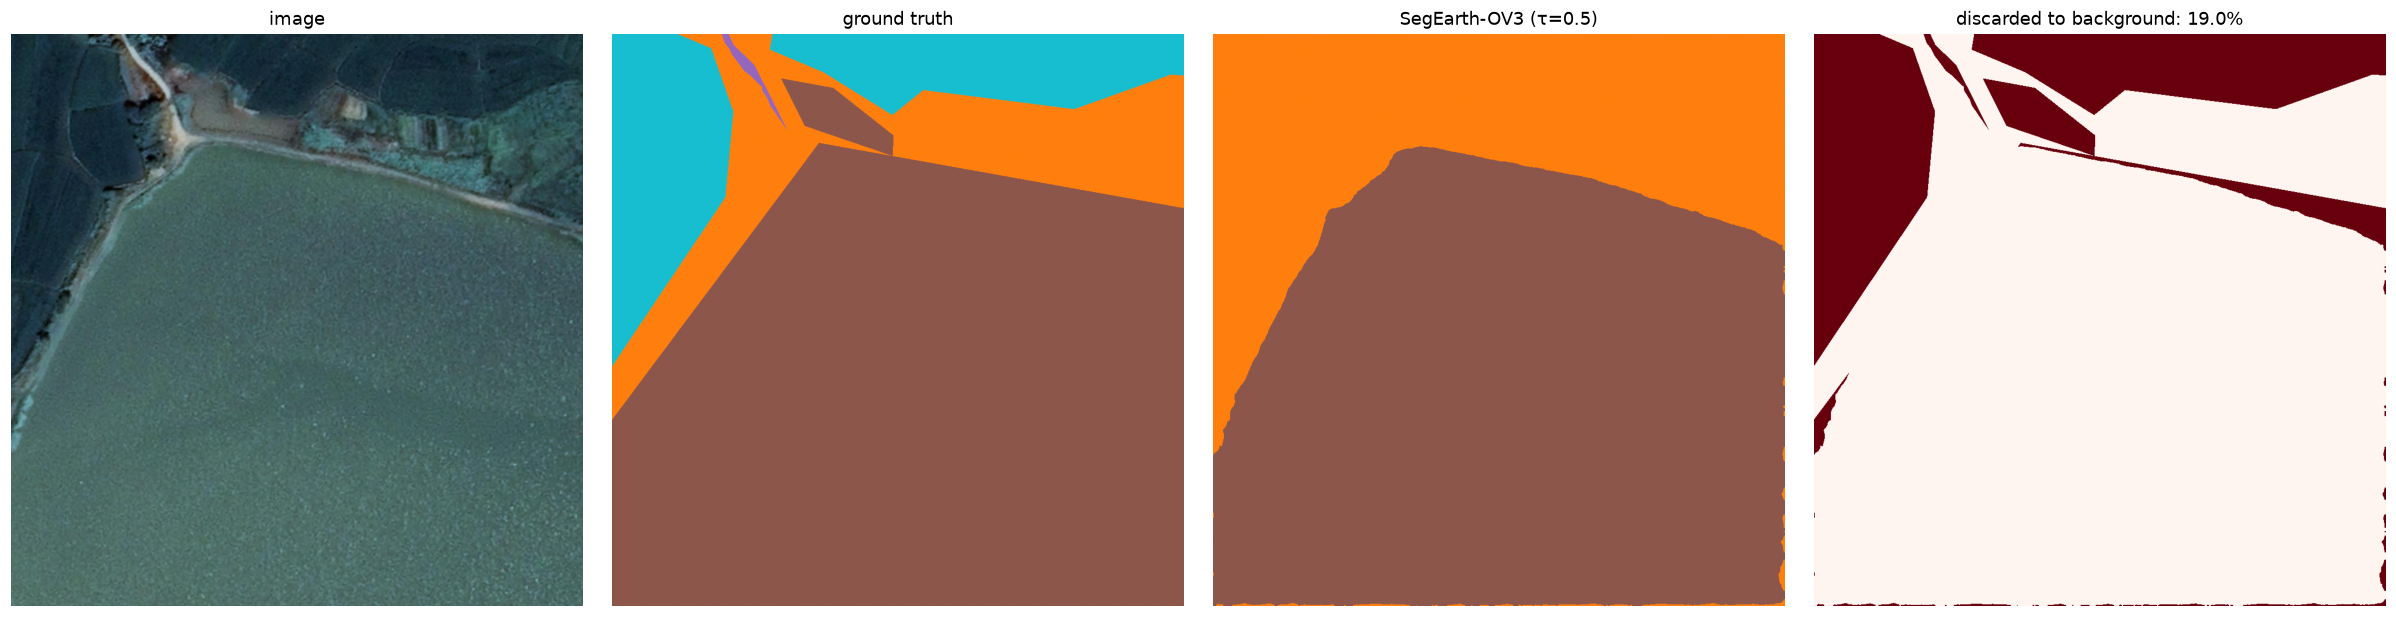
\includegraphics[width=\linewidth]{2524.png}\\
\footnotesize LoveDA tile: image / ground truth / baseline / discarded pixels.
Whole water regions dropped to \bg{}.
\end{column}
\end{columns}
\end{frame}

\begin{frame}{2. Applications --- why a cheap correction matters}
\begin{columns}[T]
\begin{column}{0.48\textwidth}
\textbf{Disaster response.} Flood extent from UAV imagery within hours. No
labelled data for the affected district; no time to train.
\vspace{0.7em}

\textbf{Renewable-energy infrastructure.} \texttt{solar panel} is a class no
land-cover benchmark contains. Supplied as two words.
\vspace{0.7em}

\textbf{Informal settlement mapping.} \texttt{tin roof}, \texttt{unpaved road},
\texttt{water tank} --- vocabulary that changes per survey.
\vspace{0.7em}

\best{Cost of our correction:} $\sim$\calibTiles{} labelled tiles, minutes of
CPU, \best{no gradient steps}. Cost of fine-tuning: thousands of tiles, a
training run, and the training-free property is lost.
\end{column}
\begin{column}{0.50\textwidth}
\vspace{0.3em}
\begin{block}{\small Measured, on Indian UAV imagery}
\small
\indTiles{} tiles, \indScenes{} openly licensed scenes, \indGSD{} --- a region
absent from all three benchmarks. Run unchanged under two class lists typed at
inference.
\end{block}
\vspace{0.2em}
\begin{itemize}\small
  \item \ok{The partition is stable under renaming:} \indFloodA{}\%
        \texttt{water} vs \indFloodB{}\% \texttt{flood water};
        \indBldgA{}\% \texttt{concrete roof} vs \indBldgB{}\% \texttt{building}.
  \item \bad{The panels are only partly found:} \indVegA{}\% of the solar-farm
        tile goes to one class when no word for them exists; \indSolarB{}\% with
        \texttt{solar panel} supplied.
\end{itemize}
\end{column}
\end{columns}
\end{frame}

\begin{frame}{2. Applications --- one scene, two vocabularies}
\begin{center}
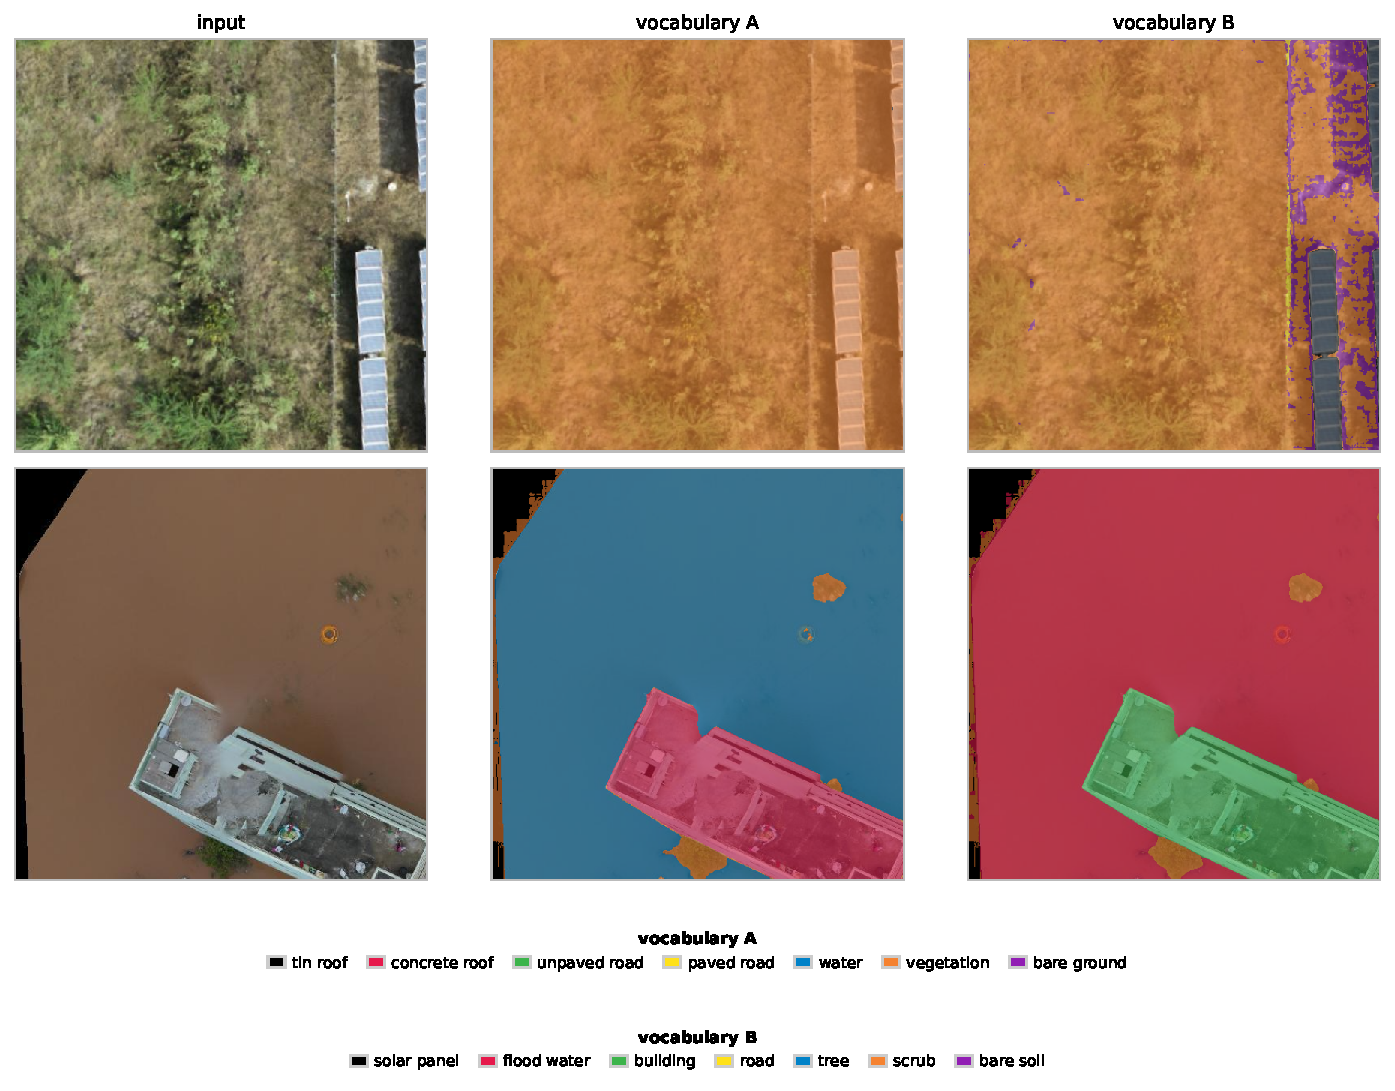
\includegraphics[height=0.70\textheight]{fig9_vocabulary.pdf}
\end{center}
\footnotesize Same weights, same forward pass; only the class list differs.
\best{Bottom:} a flooded building --- both vocabularies recover the same regions
and only the names follow the words. \best{Top:} a photovoltaic array the
settlement vocabulary has no word for. \bad{No ground truth exists for this
imagery}, so these are pixel shares, not accuracy.
\end{frame}

% ===================================================================== 3
\section{Problem Statement}
\begin{frame}{3. Problem statement --- formulation}
Let $\mathcal{C}=\{1,\dots,N\}$ be the vocabulary and $s_c(p)\in[0,1]$ the
score the pipeline assigns class $c$ at pixel $p$.

\vspace{0.6em}
\textbf{The baseline decision rule} (one global $\tau$):
\[
  \hat{y}(p)=
  \begin{cases}
    \arg\max_{c} s_c(p), & \text{if } \max_c s_c(p) \ge \tau\\[2pt]
    b \ (\textsf{catch-all}), & \text{otherwise}
  \end{cases}
\]

\vspace{0.4em}
\textbf{What we fit instead}, on a calibration set of $\sim$\calibTiles{}
labelled tiles:
\[
  \hat{y}(p)=
  \begin{cases}
    c^\star, & \text{if } s_{c^\star}(p) \ge \boldsymbol{\tau_{c^\star}}\\
    b, & \text{otherwise}
  \end{cases}
  \qquad
  c^\star = \arg\max_{c}\ \boldsymbol{w_c}\, s_c(p)
\]

\vspace{0.5em}
\begin{block}{Objective}
$(\boldsymbol{w},\boldsymbol{\tau}) \;=\; \arg\max\ \operatorname{mIoU}_{\text{real}}$
by coordinate ascent. \best{No network weights are touched.} The threshold reads
the \emph{raw} score $s_{c^\star}$, so $\boldsymbol{w}$ acts only on the
\texttt{argmax}.
\end{block}
\end{frame}

\begin{frame}{3. Why per-class $\tau$ is the \emph{complete} family --- and $w$ is not}
\textbf{Claim.} Given a fixed \texttt{argmax}, any strictly increasing per-class
recalibration $g_c$ composed with a global $\tau$ collapses to a per-class
threshold vector:
\[
  g_c(s)\ \ge\ \tau \quad\Longleftrightarrow\quad s\ \ge\ g_c^{-1}(\tau)
  \;=\;\tau_c .
\]

\vspace{0.4em}
\begin{itemize}
  \item So \best{per-class $\tau$ exhausts everything reachable by rescaling
        scores after the argmax.} Nothing in that family can beat it.
  \item Scaling \emph{before} the argmax changes \emph{which} class wins, so it
        is a \best{strictly larger family} --- it reaches the errors a threshold
        provably cannot.
\end{itemize}

\vspace{0.6em}
\begin{block}{Measured consequence (LoveDA, \S7.7)}
6.0\% of catch-all assignments are cases where the catch-all \emph{won the
argmax} at $s \ge \tau$. \bad{Lowering a threshold cannot change an argmax},
so that residual is unreachable by lever one and is exactly what lever two
addresses.
\end{block}
\end{frame}

% ===================================================================== 4
\section{Literature Survey}
\begin{frame}{4. Literature survey --- the lineage (1/2)}
\scriptsize
\begin{tabular}{@{}p{2.5cm}p{2.0cm}p{8.4cm}@{}}
\toprule
\textbf{Work} & \textbf{Venue} & \textbf{Contribution / relevance} \\
\midrule
CLIP \cite{clip} & ICML 2021 & Image--text contrastive pretraining; the origin of the open-vocabulary paradigm. \\
SAM \cite{sam} & ICCV 2023 & Promptable class-agnostic segmentation; masks without a fixed label set. \\
SAM~3 \cite{sam3} & 2025 & Presence + semantic + instance heads in one model. \best{Our backbone.} \\
MaskCLIP \cite{maskclip} & ECCV 2022 & First to extract dense predictions from CLIP by removing pooling. \\
SCLIP \cite{sclip} & 2023 & Correlative self-attention; the codebase SegEarth-OV3 derives from. \\
ClearCLIP \cite{clearclip} & ECCV 2024 & Isolates which CLIP components harm dense prediction. \\
ProxyCLIP \cite{proxyclip} & ECCV 2024 & Uses self-supervised features (DINO) as structural guidance. \\
GroupViT \cite{groupvit} & CVPR 2022 & Learns segment grouping from text supervision alone. \\
\bottomrule
\end{tabular}
\end{frame}

\begin{frame}{4. Literature survey --- direct competitors and tools (2/2)}
\scriptsize
\begin{tabular}{@{}p{2.5cm}p{2.0cm}p{8.4cm}@{}}
\toprule
\textbf{Work} & \textbf{Venue} & \textbf{Contribution / relevance} \\
\midrule
\best{SegEarth-OV} \cite{segearthov} & CVPR 2025 & Feature upsampler + global bias subtraction for RS. Defines the protocol. \\
\best{SegEarth-OV3} \cite{segearthov3} & 2025 & SAM~3 for RS OVSS: dual-head fusion + presence gating. \best{Our baseline, reproduced at 47.38 vs 47.4.} \\
\best{ConInfer} \cite{coninfer} & 2026 & GMM over DINOv3 patches fused with the VLM prior; $+2.80$ mIoU. \best{Nearest competitor --- our method \emph{composes} with it.} \\
OVRSISBench \cite{ovrsisbench} & 2026 & Unified open-vocabulary RS evaluation protocol. \\
DenseCRF \cite{densecrf} & NIPS 2011 & The classical ``use spatial context'' answer we position against. \\
CRF-as-RNN \cite{crfasrnn} & ICCV 2015 & Learned CRF inference; same family. \\
Calibration \cite{calibration} & ICML 2017 & Modern networks are systematically miscalibrated. \best{The premise we exploit.} \\
Otsu \cite{otsu} & IEEE TSMC 1979 & Classical automatic thresholding; one of our label-free baselines. \\
SLIC \cite{slic} & IEEE TPAMI 2012 & Superpixels; our region atoms. \\
LoveDA \cite{loveda} / OEM \cite{openearthmap} & NeurIPS'21 / WACV'23 & The benchmarks. \\
\bottomrule
\end{tabular}
\vspace{0.4em}
\footnotesize \textbf{16 works}; full bibliography (26 entries) in the paper.
\end{frame}

% ===================================================================== 5
\section{Research Gaps}
\begin{frame}{5. Research gaps}
\begin{enumerate}
  \item \best{The decision rule is unexamined.} Every method in this family ends
        in \texttt{argmax} + one global $\tau$, tuned per dataset. All effort
        goes into the \emph{scores}; nobody asks whether the \emph{rule} on top
        of them is the right shape.
  \vspace{0.4em}
  \item \best{The discarded residual is never quantified.} SegEarth-OV3 reports
        mIoU; it does not report that \best{29.68\%} of real-class pixels on
        LoveDA are assigned to \bg{}.
  \vspace{0.4em}
  \item \best{Catch-all classes distort the metric, in both directions.} mIoU is
        an \emph{unweighted} mean, so a catch-all owns $1/N$ of it however
        meaningless. We measure $+22.67$ inflating on one dataset and $-3.51$
        deflating on another.
  \vspace{0.4em}
  \item \best{Context is modelled visually, not semantically.} ConInfer uses a
        per-scene visual prior over patches; nobody tests a corpus-level
        \emph{semantic} class-adjacency prior. \bad{(We did --- and it fails.
        Reported as a negative with an oracle bound.)}
\end{enumerate}
\end{frame}

% ===================================================================== 6
\section{Objectives}
\begin{frame}{6. Objectives}
\begin{enumerate}
  \item \textbf{Reproduce} SegEarth-OV3 exactly, so every later number is
        measured against a baseline that runs on our hardware.
        \ok{$\checkmark$ 47.38 vs published 47.4}
  \item \textbf{Quantify} the residual the baseline discards, and test whether
        any global knob reaches it. \ok{$\checkmark$ 29.68\%; all three knobs cost more than they return}
  \item \textbf{Explain} what governs the residual across datasets, by
        intervention rather than correlation. \ok{$\checkmark$ vocabulary intervention, arity-controlled, pre-registered}
  \item \textbf{Design} a correction that trains no weights and spends the same
        supervision budget the baseline already spends.
        \ok{$\checkmark$ two levers, $+2.32$ LoveDA / $+5.67$ Potsdam}
  \item \textbf{Bound} what is achievable without labels at all.
        \ok{$\checkmark$ 12 attempts, all bounded, with a stated mechanism}
  \item \textbf{Demonstrate} on imagery and a vocabulary no benchmark covers.
        \ok{$\checkmark$ Indian UAV scenes, \indGSD{}}
\end{enumerate}
\end{frame}

% ===================================================================== 7
\section{Experimental Setup \& Results}
\begin{frame}{7. Experimental setup}
\begin{columns}[T]
\begin{column}{0.52\textwidth}
\textbf{Datasets}
\begin{itemize}\small
  \item \textbf{LoveDA} --- 1669 val tiles, $1024^2$, 0.3\,m, 7 classes,
        urban/rural split
  \item \textbf{OpenEarthMap} --- \oemTiles{} tiles, 0.25--0.5\,m, 9 classes
  \item \textbf{ISPRS Potsdam} --- 2016 tiles, 5\,cm, 6 classes
  \item \textbf{OpenAerialMap (India)} --- \indTiles{} tiles, \indGSD{},
        \bad{no ground truth}
\end{itemize}
\vspace{0.5em}
\textbf{Baselines}
\begin{itemize}\small
  \item SegEarth-OV3 (SAM~3) --- reproduced
  \item ConInfer (CLIP + DINOv3) --- run in a separate environment
  \item $\tau$ sweep, presence removal, per-class Otsu, 12 label-free rules
\end{itemize}
\end{column}
\begin{column}{0.46\textwidth}
\textbf{Protocol}
\begin{itemize}\small
  \item 5-fold cross-validation; calibration and evaluation tiles
        \best{always disjoint}
  \item Baseline recomputed on the \emph{same} held-out tiles
  \item Both metrics reported: full mIoU \emph{and} catch-all-excluded
\end{itemize}
\vspace{0.5em}
\textbf{Hardware}
\begin{itemize}\small
  \item RTX 2000 Ada, 16\,GB, 70\,W cap
  \item One LoveDA pass $\approx$ 24 min
  \item \best{Fitting the correction: minutes of CPU}
\end{itemize}
\vspace{0.5em}
\footnotesize\bad{Validation gate:} every instrumented run must still reproduce
47.37 mIoU and 29.68\% discard, or the patch changed behaviour.
\end{column}
\end{columns}
\end{frame}

\begin{frame}{7. Results --- both levers, five-fold}
\begin{center}\small
\begin{tabular}{lcccc}
\toprule
 & \textbf{LoveDA} & \textbf{Potsdam} & \textbf{OEM} & \textbf{ConInfer/LoveDA}\\
\midrule
Lever 1: per-class $\tau$   & $+1.18\pm0.45$ & $+0.59$ & $+0.30$ & \best{$+2.51\pm0.34$} \\
Lever 2: argmax scaling     & $+1.16\pm0.19$ & \best{$+4.86\pm0.35$} & --- & $-0.10$ \\
\midrule
\textbf{Total}              & \best{$+2.32$} & \best{$+5.67$} & $+0.30$ & $+2.51$ \\
Catch-all-excluded          & $+1.36$ & $+6.00$ & \best{$+1.75$} & $+1.94$ \\
Folds positive              & 5/5 & 5/5 & --- & 5/5 \\
\bottomrule
\end{tabular}
\end{center}
\vspace{0.7em}
\begin{itemize}\small
  \item \best{Two architectures} (SAM~3, CLIP+GMM), \best{three datasets},
        two operating points. \best{The claim is not about SAM~3.}
  \item \ok{Our method \emph{composes} with ConInfer}: their pipeline
        \cnRepro{} $\rightarrow$ \cnFit{} mIoU.
  \item \best{Potsdam \texttt{tree}: \treeIoUa{} $\rightarrow$ \treeIoUb{} IoU}
        (precision \treeP{}\%, recall \treeR{}\%) --- exactly the asymmetry the
        method targets.
\end{itemize}
\end{frame}

\begin{frame}{7. Results --- the method, visually}
\begin{center}
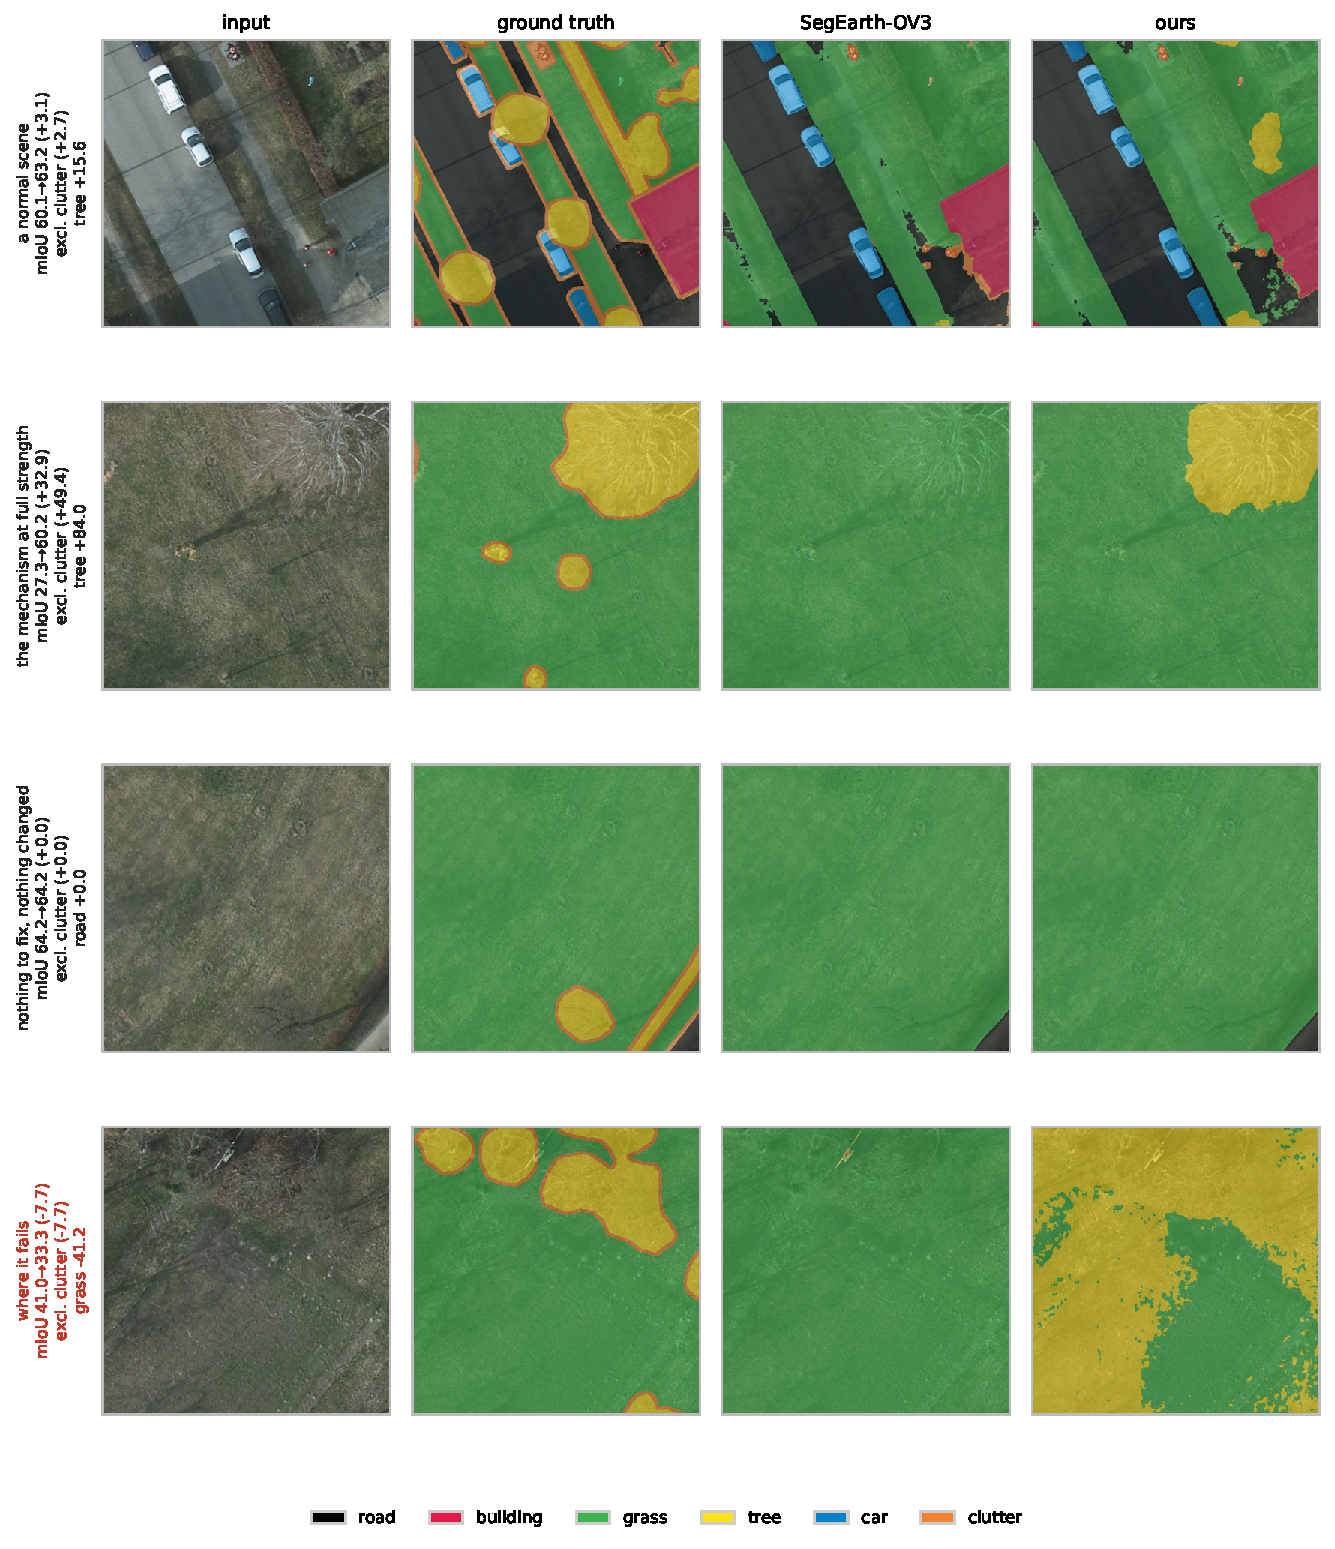
\includegraphics[height=0.72\textheight]{fig8_qualitative.pdf}
\end{center}
\footnotesize Four Potsdam tiles. Same weights, same forward pass --- only the
decision rule differs. \bad{Row four is a tile where the method LOSES 7.72
mIoU} and is included deliberately: the five-fold gain is
\scPots{}$\pm$\scPotsSD{}, an \emph{average}.
\end{frame}

\begin{frame}{7. Results --- what cannot be done without labels}
\begin{columns}[T]
\begin{column}{0.55\textwidth}
\textbf{12 label-free rules tested. All fail.}
\begin{itemize}\small
  \item Otsu, confidence percentile, presence-scaled, 8 per-class statistics,
        reachability
  \item Best: $+0.42$ against a random control's p95 of $+0.58$
  \item Oracle bound: $+1.24$
\end{itemize}
\vspace{0.6em}
\best{The mechanism, not just the failure:}
\begin{block}{}\small
Precision \emph{is} predictable without labels ($\rho=+0.943$, $p=0.017$) ---
and it does not determine the threshold ($\rho=-0.429$, $p=0.419$).
The optimal $\tau$ solves a \best{coupled multi-class IoU objective}: raising one
class's threshold moves pixels into the catch-all and changes every other
class's optimum. \best{No per-class scalar can express that.}
\end{block}
\end{column}
\begin{column}{0.43\textwidth}
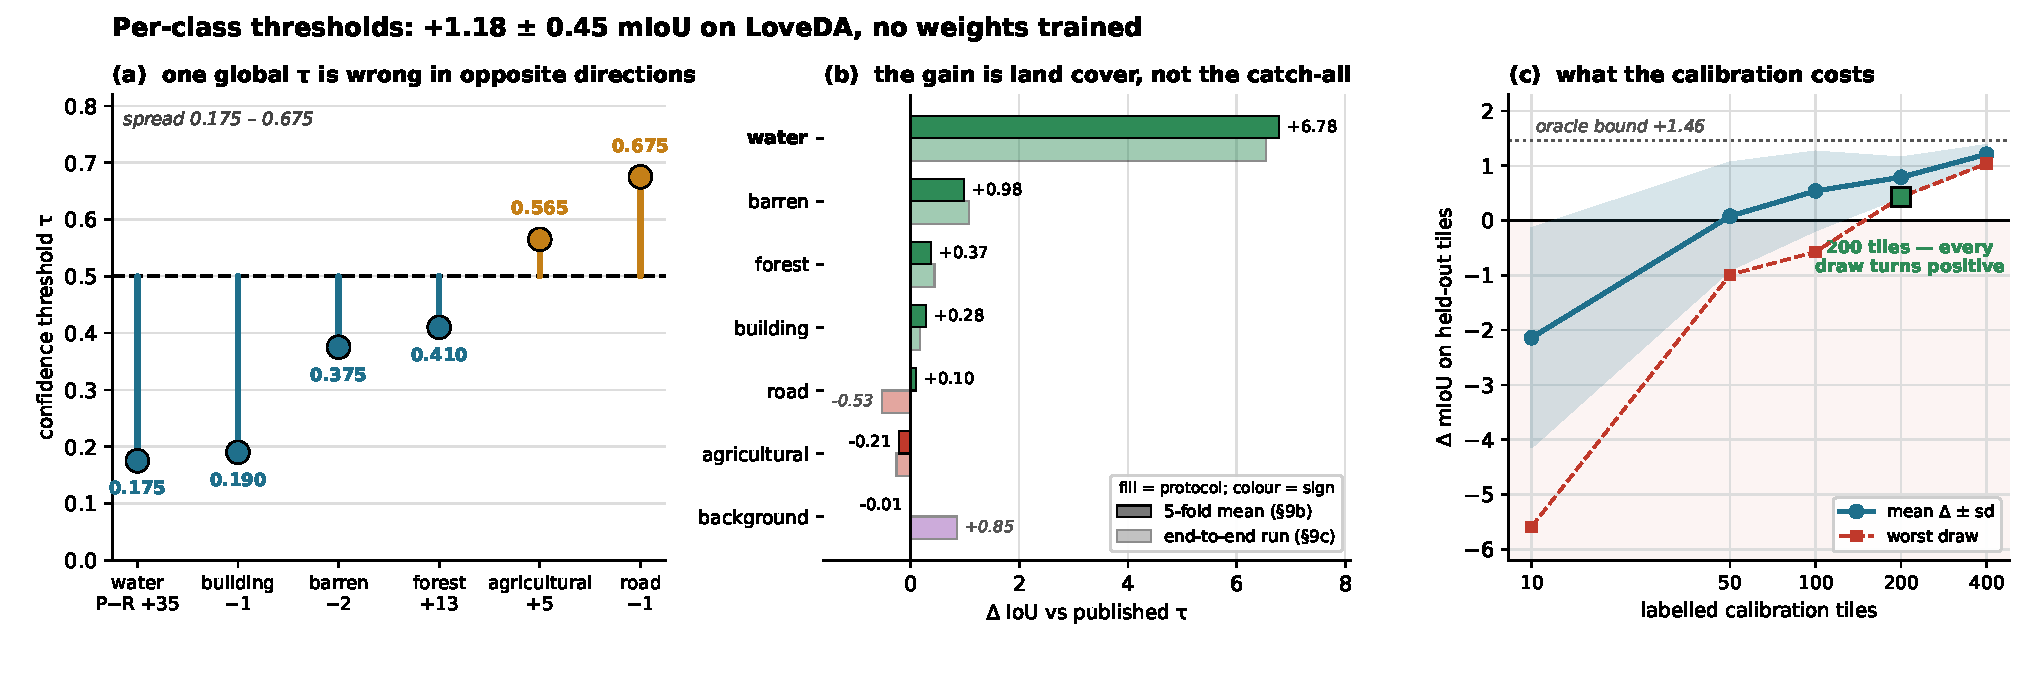
\includegraphics[width=\linewidth]{fig7_method.pdf}\\
\footnotesize Fitted thresholds span 0.175--0.675 against a single global 0.5 ---
one value is wrong for different classes \emph{in opposite directions}.
\end{column}
\end{columns}
\end{frame}

\begin{frame}{7. Honest limitations}
\begin{itemize}
  \item \bad{Thresholds do not transfer across a domain shift.} Fitted on
        LoveDA-rural, applied to urban: \bad{$-1.11$ mIoU} --- \emph{worse than
        not calibrating}. Pooling both domains also loses most of the gain.
  \item \bad{The gain is not uniform.} LoveDA rural $+2.77$, urban $+0.10$. Our
        headline is a benchmark-level figure, not a claim about every stratum.
  \item \bad{No label-free rule predicts \emph{whether} calibration will pay}
        either --- so the \calibTiles{}-tile cost buys the answer and the
        question together.
  \item \bad{The fitted vectors are constant across tiles}, so they are right on
        average and can be wrong on any individual scene (Fig.~8, row 4).
  \item \bad{ConInfer's reproduction is imperfect} --- 36.99 against a published
        39.33. We report both numbers.
\end{itemize}
\vspace{0.4em}
\footnotesize\best{Every negative in this project is reported with an oracle bound},
so the reader learns where the headroom is rather than only that we failed to
reach it.
\end{frame}

% ===================================================================== 8
\section{References}
\begin{frame}[allowframebreaks]{8. References}
\scriptsize
\bibliographystyle{ieeetr}
\bibliography{../paper/refs}
\end{frame}

\begin{frame}{Summary}
\begin{block}{What was built}
Not a new architecture. \best{Two lines of arithmetic} on top of an existing
pipeline: a per-class threshold vector and a per-class scale before the
\texttt{argmax}, fitted on $\sim$\calibTiles{} labelled tiles with
\best{no gradient steps}.
\end{block}
\begin{itemize}\small
  \item \ok{$+2.32$ LoveDA \quad $+5.67$ Potsdam \quad $+2.51$ on ConInfer's CLIP pipeline}
  \item \ok{Verified end-to-end by the official evaluator on held-out tiles}
  \item \ok{A proof that per-class $\tau$ is the complete family given the argmax}
  \item \ok{A causal experiment with pre-registered predictions}
  \item \ok{12 label-free attempts, bounded, with a stated mechanism}
\end{itemize}
\vspace{0.5em}
\centering\textbf{Target venue: IEEE Transactions on Geoscience and Remote Sensing}
\end{frame}

\end{document}
